\documentclass[a4paper]{article}

\usepackage{tecnico_relatorio}

\usepackage{textcomp}
\usepackage[hypcap]{caption} % makes \ref point to top of figures and tables
%\usepackage{rotating}
\usepackage{float}
\usepackage[]{tocbibind}
\usepackage[utf8]{inputenc}
\usepackage{graphicx}


\begin{document}
	\trSetImage{img/tecnico_logo}{6cm} % Logotipo do Técnico
\trSetSubject{Co-Projecto Hardware/Software}
\trSetType{Parte I}
\trSetTitle{Compressão de Texto Usando Codificação de Huffman}

\trSetBoxStyle{0.3}

\trSetAuthorNr{2}

\trSetAuthors
  {
  \begin{center}
  Gonçalo Ribeiro

  73294
  \end{center}
  }{
  \begin{center}
  Luís Fiolhais

  74171
  \end{center}
  }

\trSetProfessor{Prof. Horácio Neto}

\trMakeCover


	\tableofcontents
	\pagenumbering{gobble}

  \pagebreak

  \pagenumbering{arabic}
  \setcounter{page}{1}

	\section{Introdução}
  Na 1ª parte a aplicação de codificação de Huffman foi acelerada através da adição de \textit{hardware} na secção da contagem de caracteres. Nesta 2ª parte do projecto pretende-se melhorar o sistema da 1ª parte de forma a acelerar ainda mais a aplicação. Para isso é introduzido mais um factor de aceleração: a paralelização do processamento de dados, através de 4 processadores \textit{softcore} \textit{MicroBlaze}.

Da análise feita na 1ª parte observou-se que embora a aplicação tenha sido acelerada, esta não apresentava um \textit{speedup} global significativo (o \textit{speedup} das estatísticas era cerca de 400\%, mas o global era apenas de 30\%). A área escolhida na aceleração da 1ª parte foi a contagem de caracteres mas esta não era a área que despendia mais tempo de processamento, essa área pertencia à escrita do ficheiro comprimido. Nesta 2º parte para além de paralelizar as contagens com o acelerador de \textit{hardware} também foi paralelizada a secção de escrita do ficheiro comprimido.

Com este objectivo em mente, apresenta-se neste documento, a configuração do sistema usado de forma a melhorar o desempenho da aplicação e as modificações feitas ao algoritmo que permitem que a aplicação execute correctamente no sistema actualizado.

	\section{Codificação de Huffman}
	\label{sec:theory}
  \paragraph{} A codificação de Huffman é um método de compressão que consiste em encontrar uma representação alternativa --- um \emph{código} --- para cada \emph{símbolo} do alfabeto dos dados a comprimir. A compressão resulta do facto de o código escolhido para um dado símbolo ser tanto mais curto quanto maior for a frequência absoluta desse símbolo nos dados. A símbolos mais raros são atribuídos códigos mais longos. Os códigos encontrados têm uma propriedade importante: nenhum código é prefixo de outro código. Isto permite que durante o processo de descompressão não haja qualquer ambiguidade.

Os passos necessários ao algoritmo de compressão são os seguintes:

\begin{enumerate}
  \item obter as frequências absolutas de cada símbolo
  \item construir uma árvore de Huffman
  \item codificar os dados.
\end{enumerate}

O primeiro passo consiste em contar o número de ocorrências de cada símbolo até encontrar o fim do ficheiro. O segundo passo é criar uma \emph{trie} a partir das frequências obtidas no primeiro passo. Por último o ficheiro é comprimido fazendo uso da árvore criada.

O processo de criação da árvore de Huffman é:

\begin{enumerate}
  \item criar um nó para cada símbolo do alfabeto, em que se inclui a frequência desse símbolo
  \item enquanto existir mais que uma árvore
    \begin{enumerate}
    \item encontrar as duas árvores cuja raiz tem menor frequência
    \item tornar essas árvores descendentes de um novo nó, cuja frequência é a soma das frequências das raízes das duas árvores
  \end{enumerate}
\end{enumerate}

No final sobra apenas uma árvore que contém os nós correspondentes a cada símbolo. A localização desses nós na \textit{trie} dá-nos o código desse símbolo.

\subsection{Exemplo}

\paragraph{} Tome-se como exemplo o ficheiro \texttt{ABBCCCDDDD<EOF>}, em que \texttt{<EOF>} é o carácter terminador do ficheiro. As estatísticas do ficheiro são as seguintes: \texttt{\string{ A: 1, B: 2, C: 3, D: 4, <EOF>:\ 1 \string}}. A partir das estatísticas retiradas do ficheiro é gerada uma lista de prioridade. Na \autoref{fig:prio_list} apresenta-se a lista obtida.

\begin{figure}[H]
  \centering
  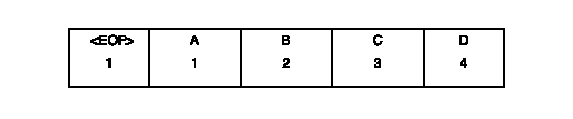
\includegraphics[width=.75\textwidth]{img/prio_list}
  \caption{Lista de prioridade gerada a partir das estatísticas}
  \label{fig:prio_list}
\end{figure}

De seguida retira-se os 2 elementos de menor prioridade da lista --- neste caso \texttt{A} e \texttt{<EOF>} --- e cria-se um novo nó que guarda a soma das suas frequências.

\begin{figure}[H]
  \centering
  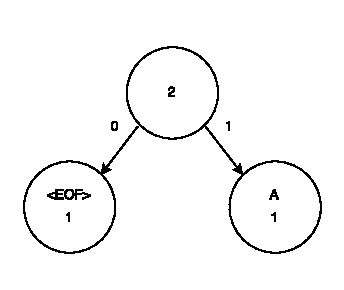
\includegraphics[width=.5\textwidth]{img/trie_1}
  \caption{Primeiro nó da árvore}
  \label{fig:trie_1}
\end{figure}

O novo nó vai ser adicionado à lista de prioridades, chamando-se \texttt{Nó 1}.

\begin{figure}[H]
  \centering
  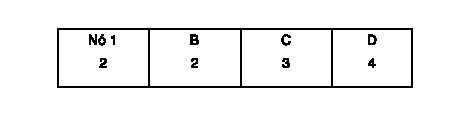
\includegraphics[width=.65\textwidth]{img/prio_list_2}
  \caption{Lista de prioridade com \texttt{Nó 1} adicionado}
  \label{fig:prio_list_2}
\end{figure}

Este processo repete-se até só existir um elemento na lista de prioridade. Na \autoref{fig:final_huffman_tree_example} encontra-se a árvore de Huffman final criada para este ficheiro.

\begin{figure}[H]
  \centering
  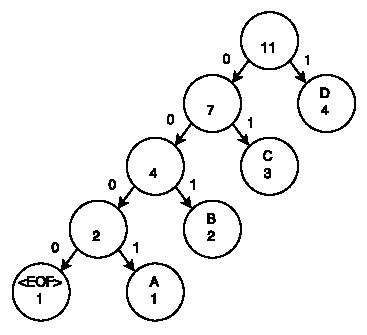
\includegraphics[width=.65\textwidth]{img/huffman_tree_example}
  \caption{Exemplo de uma árvore de Huffman}
  \label{fig:final_huffman_tree_example}
\end{figure}

Os códigos para cada carácter obtêm-se percorrendo a \textit{trie} da raiz até à folha que contem o respectivo carácter. Cada vez que se passa para um filho à esquerda adiciona-se o bit 0 à codificação; cada vez que se segue para um filho à direita adiciona-se um bit com o valor 1. Assim, por exemplo o código de \texttt{A} é \texttt{0001}, o de \texttt{C} é \texttt{01} e o de \texttt{D} é \texttt{1}. É de notar que, tal como previsto, os caracteres que ocorrem menos vezes têm códigos mais curtos.

O ficheiro comprimido seria portanto \texttt{0001 001 001 01 01 01 1 0000}. De $11 \times 8 = 88$ bits --- assumindo que é usada a representação ASCII --- passou-se a 21 bits.

No entanto, seria ainda necessário colocar no ficheiro uma representação da árvore para que o ficheiro pudesse ser descomprimido. A árvore é representada no ficheiro de saída a partir de uma pesquisa em profundidade: por cada nó interno é adicionado um 0 ao cabeçalho; quando se chega a uma folha adiciona-se um 1 seguido da representação ASCII do carácter \cite{crochemore:hal-00469994}. Este processo repete-se até se chegar à raiz da árvore. A árvore deste exemplo seria representada como: \\[5mm]
\makebox[\textwidth]{\texttt{00001 00000000 1 10000001 1 10000010 1 10000011 1 10000100}.} \par
\vspace{5mm}

 Assim, na realidade o ficheiro comprimido teria neste caso $21 + 9 + 5 \times 8 = 70$ bits, obtendo-se uma razão de compressão de $79,5\%$. Em ficheiros pequenos a inclusão da árvore tem um grande impacto, como se percebe por este exemplo. Em ficheiros grandes o \textit{overhead} da inclusão da árvore é desprezável.
 
 O ficheiro comprimido seria: \\[5mm]
\makebox[\textwidth]{\texttt{00001 00000000 1 10000001 1 10000010 1 10000011 1 10000100}} \par
\makebox[\textwidth]{\texttt{0001 001 001 01 01 01 1 0000}.} \par



	\section{Software}
  Nesta secção é descrita a implementação por software.

\subsection{Estatísticas do Ficheiro}

Para obter a frequência absoluta de cada carácter do ficheiro é feito um varrimento do ficheiro e incrementado um contador relativo ao número de ocorrências desse carácter. Isto é feito até que seja encontrado o carácter terminador. Esse carácter está definido no programa como \texttt{FILE\_END\_CODE}. Ao longo desta parte do trabalho tem-se considerado como terminador o carácter \texttt{0x00}.

A razão pela qual é preciso escolher um carácter como terminador prende-se com o facto de não termos um sistema operativo a correr no MicroBlaze. Caso tivesse um sistema operativo, ele podia notificar o programa quando não houvesse mais conteúdo para ler.

A complexidade desta fase do algoritmo é linear com o tamanho do ficheiro. Antes de se passar à construção da árvore, é construído um vector com pares (carácter, contagem), que não inclui caracteres com frequência absoluta nula. Na construção da árvore são portanto considerados apenas caracteres com pelo menos uma ocorrência. Isto resulta numa árvore mais pequena (menor \textit{overhead} no ficheiro comprimido) e torna a construção da árvore mais rápida.

\subsection{Árvore}

Tal como visto na Secção~\ref{sec:theory} uma operação muito frequente durante a construção da árvore de Huffman é encontrar as duas raízes que em cada momento têm menor frequência absoluta. De forma a acelerar estas procuras, fez-se a implementação da árvore recorrendo a um acervo (\textit{heap}) que contém apontadores para os nós da árvore. O acervo é construído com complexidade $O(n)$, permite remoção do elemento com menor frequência em $O(log\ n)$ e inserção também $O(n)$, em que $n$ é o número de elementos, sendo que neste caso temos $n \leq 256$.

Por cada dois elementos (nós) que são removidos do acervo é adicionado um novo com frequência igual à soma das frequências dos que foram removidos. Os nós removidos são depois ``pendurados'' debaixo do novo nó. Assim sendo, cada elemento do acervo é na verdade uma árvore. Quando o acervo tiver apenas um elemento temos certeza de que esse constitui a árvore de Huffman. Note-se que por cada dois elementos que são removidos é adicionado apenas um, pelo que construir a árvore de Huffman demora, no máximo, 255 passos.

\subsection{Ficheiro de Saída}

Percorrendo a árvore de Huffman é possível obter o código que corresponde a cada carácter. De forma a optimizar o processo de codificação do ficheiro, começa-se por percorrer a árvore com o objectivo de construir uma tabela indexada pelos caracteres, e que em cada posição contem um par (código, comprimento), em que \emph{comprimento} é o número de bits do código. Recorrendo a esta tabela é agora possível aceder ao código de cada carácter em tempo constante.

Para codificar o ficheiro resta agora substituir os caracteres do ficheiro pelos seus códigos. Esta operação não é assim tão trivial visto que a unidade mínima de memória que é possível endereçar é o byte. Por este motivo é necessário codificar vários caracteres para construir cada byte do ficheiro de saída. Isto implica uma série de operações lógicas (\textit{shifts} e \textit{ORs}) e aritméticas que demoram uma quantidade apreciável de tempo, como se pode notar na secção~\nameref{sec:results}.


  \section{Sistema}
  O sistema opera a 75~MHz com 4 \textit{MicroBlazes} com a seguinte configuração:
o processador mestre possui uma memória local de 64~kB, 2 \texttt{AXI~Timers} de 32 bits ligados em cascata --- que resulta num \textit{timer} de 64 bits --- e uma \textit{cache} de 8~kB de dados. Os restantes processadores, escravos, possuem uma memória local de 16~kB com a mesma configuração de \textit{cache} (ambas as \textit{caches} apresentam uma política \textit{write-through}). São usadas duas memórias internas, uma de 4~kB e outra de 16~kB. A primeira está ligada ao \textit{bus} \texttt{AXI Lite} --- para não ter cache; a segunda ao \textit{bus} \texttt{AXI} --- de forma a tomar partido da cache --- é usada para guardar a tabela de conversões, de carácter para representação de Huffman.

Em suma, o sistema é constituído pelos seguintes componentes:

\begin{itemize}
	\item 1 \textit{MicroBlaze} mestre
    \begin{itemize}
		\item 64~kB de memória local
        \item 8~kB de \textit{cache} de dados; 64~B de \textit{cache} de instruções
	\end{itemize}
    \item 3 \textit{MicroBlazes} escravos
    \begin{itemize}
		\item 16~kB de memória local
        \item 8~kB de \textit{cache} de dados; 64~B de \textit{cache} de instruções
	\end{itemize}
    \item 1 memória interna de 4~kB, sem \textit{cache}
    \item 1 memória interna de 16~kB, com \textit{cache}
    \item 1 memória externa de 128~MB, com \textit{cache}
    \item 1 temporizador AXI de 64 bits (2 de 32, em cascata)
    \item 1 módulo UART
\end{itemize}


A memória externa está ligada através do \textit{bus} AXI4, de maneira a tomar partido da \textit{cache} de dados e instruções. A memória interna que não está ligada à cache é usada da seguinte forma:

\begin{itemize}
\item Primeiros 4 bytes para sincronizar os vários processadores;
\item Endereços de 0x4 a 0x403 são usados pelo processador 1 para partilhar contagens com o processador 0;
\item Endereços de 0x404 a 0x803 são usados pelo processador 2 para partilhar contagens com o processador 0;
\item Endereços de 0x804 a 0xC03 são usados pelo processador 3 para partilhar contagens com o processador 2;
\item As restantes posições não são utilizadas.
\end{itemize}


O programa usado no processador mestre usa cerca de 54~kB e os restantes cerca de 9~kB. Ao processador mestre foi atribuída uma \textit{stack} de 10~kB, pois a pesquisa na árvore é feita recursivamente. Como no pior caso a árvore tem 256 níveis podem ser ocupados aproximadamente $256 \times (4 + 4 + 4) = 3072$ B em \textit{stack}, visto que cada chamada recursiva usa dois ponteiros mais um \texttt{char} e \texttt{short} --- assumindo que são usados 4 bytes devido a alinhamentos. Contabilizando outros dados que são colocados na \textit{stack} por cada chamada, estima-se que o tamanho da \textit{stack} possa chegar a cerca de 5~kB. Para ter margem de segurança definiu-se no \textit{linker script} uma \textit{stack} com o número redondo de 10~kB. Os restantes processadores usam 1~kB de \textit{stack} e de \textit{heap}, visto que o processamento feito não necessita de uma grande quantidade de memória.

Não foi usada qualquer optimização por parte do compilador (\texttt{-O0}).

Alguns valores relativos à ocupação do sistema (valor absoluto e percentagem de ocupação) são:


\begin{verbatim}
            Slice registers               8 652       15 %
            Slice LUTs                   11 981       43 %
               used as Memory             1 855
            occupied Slices               4 355       63 %
            LUT Flip Flop pairs used     13 690
            RAMB16BWERs                      86       74 %
            RAMB8BWERs                        0        0 %
            DSP48A1s                         12       20 %
\end{verbatim}


	\section{Acelerador}
	\label{sec:accelerator}
  \paragraph{} Nesta secção propõem-se um circuito para acelerar a contagem de caracteres do ficheiro.

\subsection{Motivos}
  \paragraph{} As partes mais demoradas da implementação são a contagem da frequência absoluta dos caracteres e a codificação do ficheiro. O tempo da contagem cresce linearmente com o tamanho do ficheiro. Já a codificação do ficheiro aparenta também crescer linearmente com o tamanho do ficheiro, mas a relação deve ser mais complicada: nesta fase é preciso voltar a ler o ficheiro de entrada (tempo linear) e montar os bytes do ficheiro e saída. O tempo que se demora a montar bytes deverá ser tanto maior quanto melhor for a compressão conseguida: por exemplo, para um ficheiro em que haja ocorrências apenas de um carácter serão necessárias 8 iterações que envolvem \textit{shifts}, \textit{ORs} e operações aritméticas para montar cada byte. No caso patológico --- em que não se consegue qualquer compressão com codificação de Huffman --- de todos os 256 caracteres ocorrem no ficheiro, com frequências iguais, cada código teria 8 bits pelo que para montar cada byte bastaria 1 iteração.

  Tendo em conta os resultados da \autoref{tab:time_software} escolhe-se desenhar hardware para acelerar as estatísticas do ficheiro.

  \subsection{Datapath}

  \begin{figure}[H]
    \centering
    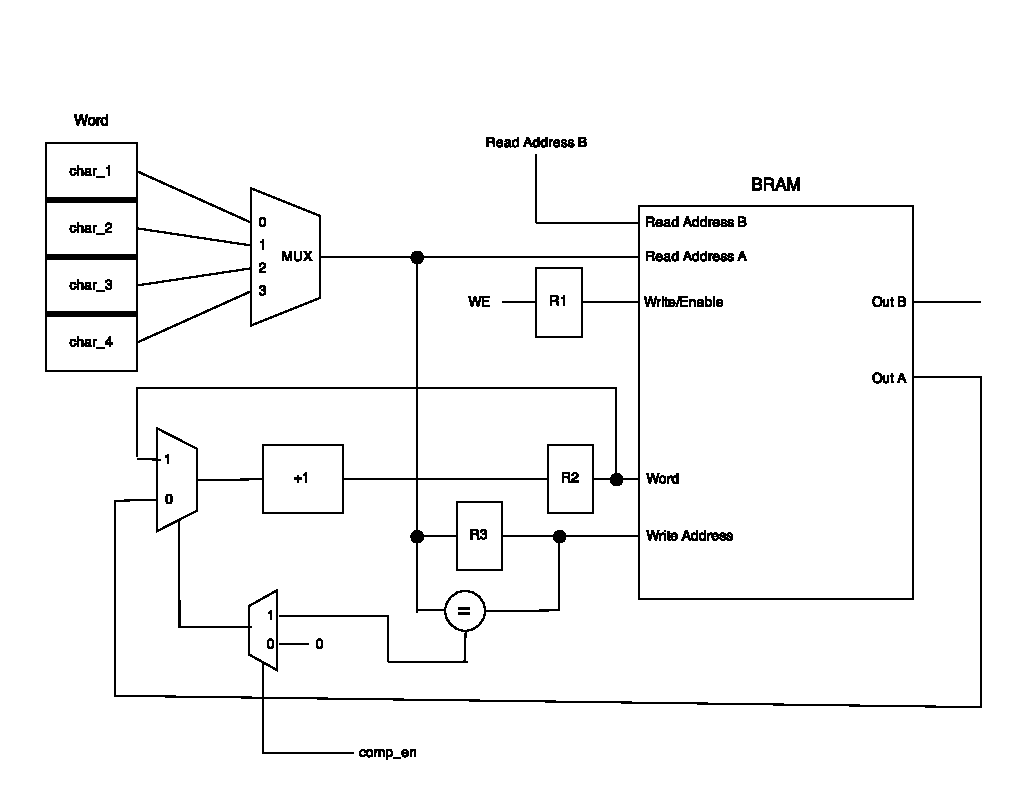
\includegraphics[width=1.0\textwidth]{img/hw_datapath}
    \caption{Datapath do acelerador}
    \label{fig:hw_datapath}
  \end{figure}

  \paragraph{} A \autoref{fig:hw_datapath} mostra a datapath usada no acelerador. Esta recebe 4 caracteres porque cada caracter são 8 bits e a \texttt{FSL} transporta 32 bits, contém um incrementador e uma \texttt{BRAM} de 256 posições com 16 bits cada (512KB). O próprio caracter endereça a \texttt{BRAM}, o valor lido é incrementado e de seguida é guardado na \texttt{BRAM}. Caso exista dois caracters repetidos na palavra em vez de ser incrementado o valor da \texttt{BRAM} é incrementado o valor da contagem calculado anteriormente.

\subsection{Máquina de Estados}
  \begin{figure}[H]
    \centering
    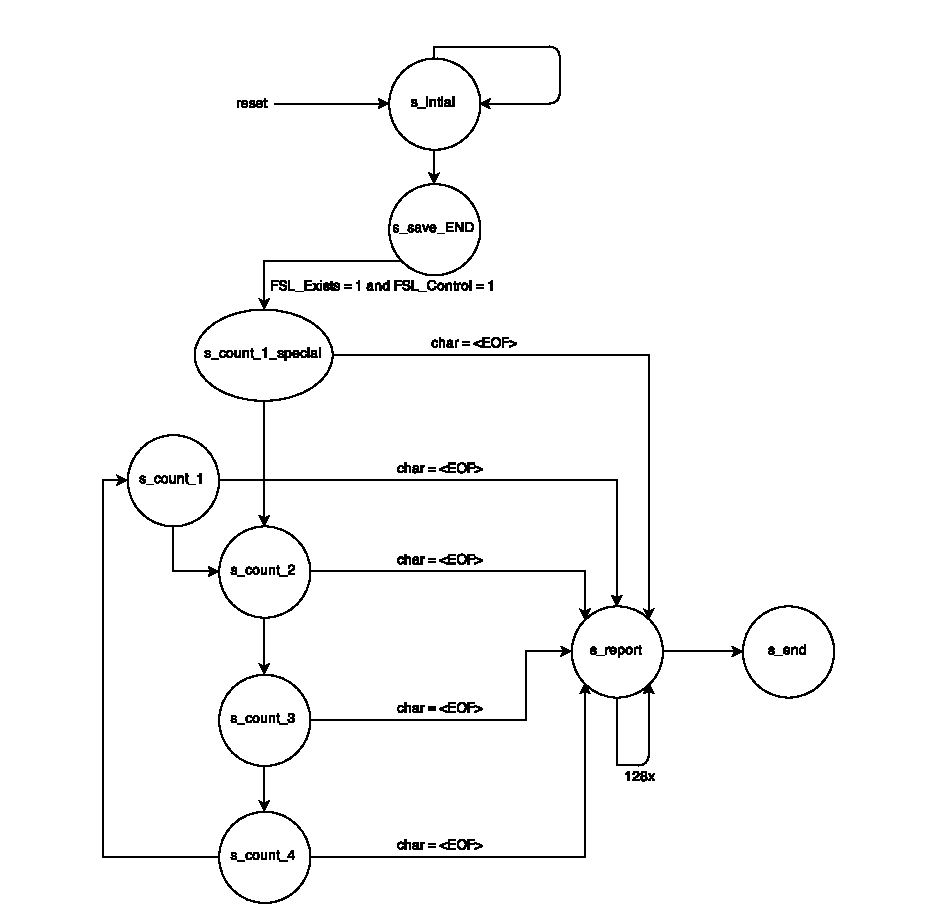
\includegraphics[width=1.0\textwidth]{img/fsm}
    \caption{Máquina de Estados do acelerador}
    \label{fig:hw_fsm}
  \end{figure}

  \paragraph{} A máquina de estados apresentada na \autoref{fig:hw_fsm} é iniciada com o sinal \texttt{FSL\_Reset} e fica presa no estado \texttt{s\_initial} até dados se encontrarem na \texttt{FSL} e ter recebido o caracter terminador (\texttt{<EOF>}). Este é enviado em simultâneo com o sinal de controlo.

  O primeiro estado de contagem, \texttt{s\_count\_1\_special}, é especial pois não tem nenhum caracter anterior com que comparar. Os restantes estados têm que comparar com o caracter anterior e geram a palavra de selector do \texttt{MUX} conforme o caracter que pretendem ler.

  Quando o caracter terminador é encontrado o próximo estado vai ser o \texttt{s\_report}. Neste estado é escrito o conteúdo total da \texttt{BRAM} para o \texttt{FSL}, como cada contagem são 16 bits é possível escrever 2 contagens em simultâneo, repetindo-se 128 vezes.


	\section{Resultados}
	\label{sec:results}
  Nesta seccção são apresentados os resultados temporais e de compressão de vários ficheiros de exemplo. Nos resultados temporais compara-se o desempenho da implementação puramente em software com a solução com aceleração por hardware.

\subsection{Temporais}

  Na \autoref{tab:time_software} estão patentes os tempos de execução da implementação totalmente em software do algoritmo de compressão. Pode-se notar que existem dois passos que correm em tempo praticamente constante: construir a árvore e transformar a árvore numa tabela. Embora o tempo destes passos não seja constante, é proporcional ao número de caracteres distintos existentes no ficheiro; e consequentemente é limitado superiormente. Este é o motivo pelo qual as operações sobre a árvore para o ficheiro \texttt{pdf} demoram menos tempo do que para \texttt{teste}: o ficheiro \texttt{teste} tem 25 caracteres distintos enquanto que \texttt{pdf} tem apenas 14, logo as operações sobre a árvore demoram mais tempo para o primeiro.

  O acelerador é descrito na Secção~\ref{sec:accelerator}. O tempo de execução das estatísticas por software é comparado ao da solução hardware/software na \autoref{tab:time_hardware}. Através desta tabela notamos que a aceleração conseguida é significativa: a parte do algoritmo que foi acelerada por hardware é agora cerca de 4 vezes mais rápido. Isto resulta em que a solução que incorpora o acelerador é 1,32 vezes mais rápida do que a solução puramente por software, como se verifica pela\autoref{tab:speedup_total}. Para os ficheiros mais pequenos não houve aceleração, ou a mesma foi escondida por os tempos medidos não serem mais precisos.
  
  \paragraph*{Nota:} a compilação foi feita com a \textit{flag} \texttt{-o0}, em todos os casos.


  \begin{table}[p]
    \caption{Tempo de execução de cada parte do algoritmo, por software}
    \centerline
    {
      \begin{tabular}{|c|r|c|c|r|r|}
        \hline
        \textbf{Ficheiro}                             &
        \multicolumn{1}{c|}{\textbf{Estatísticas}}    &
        \textbf{Construir Árvore}                     &
        \textbf{Árvore $\rightarrow$ Tabela}          &
        \multicolumn{1}{c|}{\textbf{Codificação}}     &
        \multicolumn{1}{c|}{\textbf{Tamanho}} \\
        \hline
        \hline
        tmp       & \ 1 ms    & \ 0 ms & 0 ms & \ 0 ms    & 14 B    \\ \hline
        teste     & \ 1 ms    & \ 5 ms & 1 ms & \ 0 ms    & 28 B    \\ \hline
        pdf       & \ 1 ms    & \ 3 ms & 0 ms & \ 1 ms    & 44 B    \\ \hline
        read\_me  & 21 ms     & 12 ms  & 1 ms & 43 ms     & 2981 B  \\ \hline
        alice     & 1248 ms   & 32 ms  & 3 ms & 2611 ms   & 174 KB  \\ \hline
        BIG\_READ & 76584 ms  & 32 ms  & 3 ms & 159882 ms & 10,4 MB \\
        \hline
      \end{tabular}
    }

    \label{tab:time_software}
  \end{table}



  \begin{table}[p]
    \centering
    \caption{Comparação das contagens (estatísticas) em software\\ e em hardware/software. Respectivo \textit{speedup}}

    \begin{tabular}{|c|r|r|r|}
      \hline
      \textbf{Ficheiro}                                 &
      \multicolumn{1}{c|}{\textbf{Software}}            &
      \multicolumn{1}{c|}{\textbf{Hardware/Software}}   &
      \multicolumn{1}{c|}{\textbf{Speedup}}       \\ \hline \hline
      tmp        & \ 1 ms     & 1 ms     & 1,00   \\ \hline
      teste      & \ 1 ms     & 1 ms     & 1,00   \\ \hline
      pdf        & \ 1 ms     & 1 ms     & 1,00   \\ \hline
      read\_me   & 21 ms      & 6 ms     & 3,50   \\ \hline
      alice      & 1248 ms    & 314 ms   & 3,97   \\ \hline
      BIG\_READ  & 76584 ms   & 19231 ms & 3,98   \\
      \hline
    \end{tabular}
    \label{tab:time_hardware}
  \end{table}


  \begin{table}[p]
    \caption{Tempo de execução total e \\\textit{speedup} global para cada ficheiro}
    \centerline
    {
      \begin{tabular}{|c|r|r|c|}
        \hline
        \textbf{Ficheiro}                                &
        \multicolumn{1}{c|}{\textbf{Hardware}}           &
		\multicolumn{1}{c|}{\textbf{Hardware/Software}}  &
        \textbf{Speedup}                            \\ \hline \hline
		tmp       &      1 ms   &      1 ms & 1,00  \\ \hline
        teste     &      7 ms   &      7 ms & 1,00  \\ \hline
        pdf       &      5 ms   &      5 ms & 1,00  \\ \hline
        read\_me  &     77 ms   &     62 ms & 1,24  \\ \hline
        alice     &   3894 ms   &   2960 ms & 1,32  \\ \hline
        BIG\_READ & 236501 ms   & 179148 ms & 1,32  \\
        \hline
      \end{tabular}
    }

    \label{tab:speedup_total}
  \end{table}



  \subsection{Compressão}

  A \autoref{tab:compression} apresenta o tamanho dos ficheiros de teste após compressão, bem como os seus tamanhos originais.

  \begin{table}[p]
    \centering
    \caption{Compressões conseguidas para os ficheiros de teste}
    \begin{tabular}{|c|r|r|r|}
        \hline
        \textbf{Ficheiro}                                 &
        \multicolumn{1}{c|}{\textbf{Original}}            &
        \multicolumn{1}{c|}{\textbf{Comprimido}}          &
        \multicolumn{1}{c|}{\textbf{Rácio}}\\ \hline \hline
        tmp        &  13,0  B    &  11,00 B          & 85,0\%     \\ \hline
        teste      &  27,0  B    &  49,00 B          & 181,5\%    \\ \hline
        pdf        &  43,0  B    &  39,00 B          & 90,7\%     \\ \hline
        read\_me   &  3,0  KB    &  1,62 KB          & 54,0\%     \\ \hline
        alice      &  174,0 KB   &  103,79 KB        & 59,6\%     \\ \hline
        BIG\_READ  &  10,4 MB    &  5,99 MB          & 57,6\%     \\
        \hline
    \end{tabular}
    \label{tab:compression}
  \end{table}

  A partir destes resultados pode-se afirmar que todos os ficheiros apresentam uma boa razão de compressão, à excepção do ficheiro \texttt{teste}. Este é um caso extremo do algoritmo de Huffman: neste caso o ficheiro possui uma variedade significativa de caracteres, o que aliado ao seu tamanho reduzido torna difícil a sua compressão visto que a árvore gerada é relativamente grande e, consequentemente, o cabeçalho gerado para o ficheiro comprimido representa um grande \textit{overhead}. Por este motivo, o algoritmo, em vez de comprimir o ficheiro expandiu-o em 81,5\%.


	\section{Conclusão}
  \paragraph{} Como demonstrado obteve-se um compressor de texto com codificação de Huffman a funcionar num \textit{MicroBlaze} numa \textit{Spartan-6}. Também se averiguou a viabilidade da adição de um acelerador nas contagens de caracteres e verificou-se que este acelera o processamento em várias ordens de grandeza para ficheiros de dimensão considerável, enquanto que em ficheiros de dimensão mais pequena o efeito do acelerador não é sentido.

Através destes resultados pode-se afirmar que ainda há margem para melhorar o desempenho da aplicação e a \autoref{tab:time_software} demonstra que o módulo de codificação do ficheiro ainda ocupa uma grande percentagem do tempo de execução, pelo que este módulo vai ser implementado em hardware na 2ª parte do projecto.


  \pagebreak

  \listoffigures
  \listoftables

	% references
  \begin{thebibliography}{9}

  \bibitem{rocha13a}
   Rui Manuel Rodrigues Rocha,
   \emph{Network Embedded Systems: Node Architecture},
   Universidade Técnica de Lisboa - Instituto Superior Técnico,
   2013.

\end{thebibliography}


  \pagebreak

  % anexo com as tabelas raw do acelerador
  \appendix

  \section{Tabela Auxiliar}

  \begin{table}[h]
    \caption{Tempo de execução de cada parte do algoritmo, \\com acelerador por hardware}

    \centerline
    {
      \begin{tabular}{|c|r|c|c|r|}
        \hline
        \textbf{Ficheiro}                             &
        \multicolumn{1}{c|}{\textbf{Estatísticas}}    &
        \textbf{Construir Árvore}                     &
        \textbf{Árvore $\rightarrow$ Tabela}          &
        \multicolumn{1}{c|}{\textbf{Codificação}}         \\ \hline \hline
        tmp       & \ 1 ms    & \ 0 ms & 0 ms & \ 0 ms    \\ \hline
        teste     & \ 1 ms    & \ 5 ms & 1 ms & \ 0 ms    \\ \hline
        pdf       & \ 1 ms    & \ 3 ms & 0 ms & \ 1 ms    \\ \hline
        read\_me  & 6 ms      & 12 ms  & 1 ms & 43 ms     \\ \hline
        alice     & 314 ms    & 32 ms  & 3 ms & 2611 ms   \\ \hline
        BIG\_READ & 19231 ms  & 32 ms  & 3 ms & 159882 ms \\
        \hline
      \end{tabular}
    }

    \label{tab:time_hardware_all}
  \end{table}



\end{document}
